\documentclass[letterpaper]{article}
\usepackage[utf8]{inputenc}
\usepackage{float}
\setlength\parindent{0pt}
\usepackage{graphicx}
\graphicspath{{./figures/}}

\newcommand{\p}{\vspace{1em}\par}		% macro to start new paragraph

\author{David De Lille}
\title{Offensive Computer Security: Summary 1}

\begin{document}
\maketitle

\section{Risk}
Risk = Threat x Vulnerability

\begin{quote}
``Risk is a function of the likelihood of a given thread-source's exercising a particular potential vulnerability, and the resulting impact of that adverse event on the organisation.''
\end{quote}

Threat: consequences of bad thing happening\\
Vulnerability: probability of bad thing happening

\section{Hacking versus Penetration testing}
The difference is: permission. Penetration testing without permission is illegal.

\section{History of Disclosure}
\setcounter{subsection}{-1}	% start counting subsections from 0
\subsection{No disclosure [1950-1988]}
\subsection{Mailing lists [1988-1993]}
Security is only discussed on invite-only mailing lists. Security researchers seen as evil, and vendors don't care. Mailing lists were easily leaked. Everything is buy-at-your-own-risk.

\subsection{Full Disclosure [1993-2002]}
This was a (controversial) reaction to vendors being unwilling to solve security problems, in order to force them to act. Researchers would disclose security problems to everyone (good and bad).
The result was a constant a race between exploiters and patchers. This is still a problem for start-ups that don't have the resources for specialized security personnel. It didn't reduce the amount of attacks.

\subsection{Responsible Disclosure [2002-2010]}
Process submitted to IETF. Similar to Full Disclosure, but researchers should wait to release info until the vendor can patch the problem. The problem was that this places the  responsibility to fix the problem on the researcher, rather than the vendor.

\subsection{Coordinated Vulnerability Disclosure [2010-present]}
Vendors promise not to sue researchers, and accept responsibility for the problems. Vendorsec mailing lists were attempted, but were again broken/leaked.\\
Delayed disclosure = give vendor a certain amount of time to patch before doing full disclosure. Abused by researchers at conferences to gain glory.\\
Bug bounties are programs offered by certain companies that grant cash rewards for discovering bugs.

\section{Penetration testing cycle}
\begin{figure}[H]
\centering
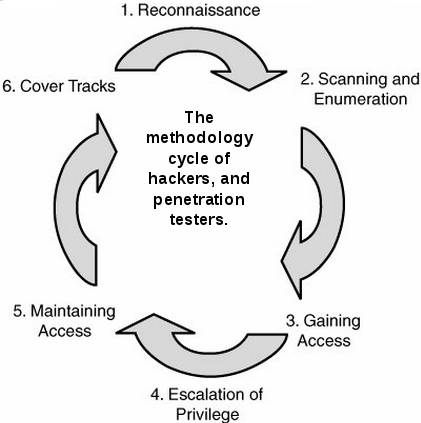
\includegraphics[scale=0.71]{penetration_testing_cycle.png}
\end{figure}
(Note: cycle can restarted at any point.)

\setcounter{subsection}{-1}	% start counting subsections from 0
\subsection{Prior}
Discuss the details of the engagement with the client:
\begin{itemize}
\item what: which targets, what is off limits, what kind of threat model (e.g. insider threat, ex-employee), BYOD?
\item how: physical access?, social engineering?, covert/overt?
\item when: timeline of the pentest
\item report: what kind of report are they expecting?
\end{itemize} 
	
\subsection{Reconnaissance}
Gathering intelligence on the target(s). Two types of intel: OSINT and HUMINT.
 
\p OSINT (open source intelligence):
\begin{itemize}
\item search engines: URLs, filetypes, devices (http://www.shodanhq.com/)
\item company website
\item public records
\item social media
\item way-back-machine
\end{itemize}

HUMINT (human intelligence):
\begin{itemize}
\item phone
\item physical access
\end{itemize}
	
\subsection{Scanning and Enumeration}
The goal is to identify the \textbf{attack surface}, by scanning ways to get in and finding new ways. Jump back to Reconnaissance step if needed. Finally, find vulnerabilities in the attack surface.
	
\subsection{Gain access}
Exploit vulnerabilities to break in:
\begin{itemize}
\item Social Engineering (easiest way by far)
\item web app exploitation
\item pivoting from 3rd party
\item network app exploitation
\item malicious USB
\item etc
\end{itemize}
	
\subsection{Privilege Escalation}
Increase capabilities by:
\begin{itemize}
\item password cracking
\item SUID exploits
\item sandbox escape
\item keylogging
\item social engineering
\item etc
\end{itemize}
	
\subsection{Maintain access and Post Exploitation}
Complete the actual goal of attack, which can include:
\begin{itemize}
\item going after money/data/users/intellectual property
\item installing a backdoor
\item expanding control (e.g. passwords, pivoting to 3rd party)
\item erasing logs
\end{itemize}

\section{Threat models}
\begin{itemize}
\item Attacker centric: what are his goals and how can he achieve them
\item Software centric: design review (step through and evaluate each part)
\item Asset centric: start from pot o' gold
\end{itemize}

\section{Categories of Threats}
\begin{figure}
\centering
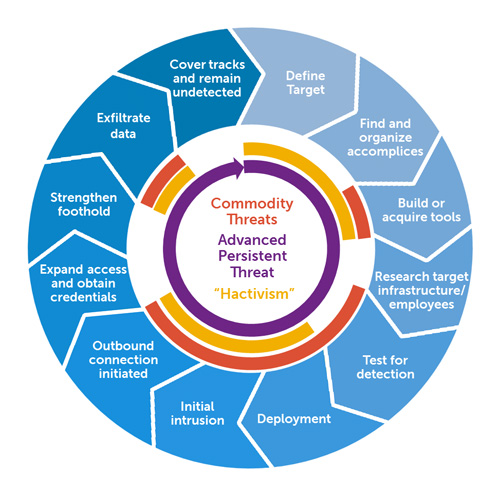
\includegraphics[scale=0.5]{Advanced_persistent_threat_lifecycle.jpg}
\caption{Attacker life cycle}
\end{figure}

\begin{itemize}
\item Advanced Persistent Threat (APT): most powerful hackers (potentially state-funded)
\item Hacktivism: LulzSec, Anonymous, etc.
\item Commodity threats: as capable as hactivists, but fewer in numbers
\end{itemize}

\section{Attacker goals}
What are the bad guys after:
\begin{itemize}
\item money/data/users/intellectual property
\item critical infrastructure
\item enemies/political dissidents
\item credit cards/financial data
\item password (hashes)
\item sabotage
\item pivoting to 3rd party
\item long term backdoors
\item 4 teh lulz
\end{itemize}

\section{Asymmetric advantage attacker}
Attackers only need to find one hole; defenders need to stop everything.
\p Bad guys also have distinct advantages over pentesters:
\begin{itemize}
\item can be completely anonymous (proxy, spoofing)
\item attack BYOD/significant other
\item attack partners
\item blackmail, \$5 wrench
\item widely available crime kits
\item can break laws
\end{itemize}

\section{Other Notes}
\begin{itemize}
\item Physical access = game over
\item Its important to know how to communicate security  
\end{itemize}
\end{document}